% Copyright 2025 Fausto Spoto
%
% Licensed under the Apache License, Version 2.0 (the "License");
% you may not use this file except in compliance with the License.
% You may obtain a copy of the License at
%
%    http://www.apache.org/licenses/LICENSE-2.0
%
% Unless required by applicable law or agreed to in writing, software
% distributed under the License is distributed on an "AS IS" BASIS,
% WITHOUT WARRANTIES OR CONDITIONS OF ANY KIND, either express or implied.
% See the License for the specific language governing permissions and
% limitations under the License.

\documentclass[11pt]{beamer}  %% versione proiettore
%%\documentclass[11pt,handout]{beamer} %% versione stampa
\usepackage{lucidiJb-2ed}

\usepackage{mathtools}
\usepackage{relsize}
\usepackage[normalem]{ulem}

\mode<article>
{
  \usepackage{fullpage}
  \usepackage{hyperref}
}

\mode<presentation>
{
  \setbeamertemplate{background canvas}[vertical shading][bottom=red!10,top=blue!10]
  \usetheme{Course}
  \usefonttheme[onlysmall]{structurebold}
}

\subtitle{Saint-Denis, R\'eunion, 13/3/2025}
\title{Blockchain and its Energy Cost}
\institute{Universit\`a di Verona, Italy}
\date{March 2025}

\setbeamercovered{invisible}

\def\codesize{\smaller}
\def\<#1>{\codeid{#1}}
\newcommand{\codeid}[1]{\ifmmode{\mbox{\codesize\ttfamily{#1}}}\else{\codesize\ttfamily #1}\fi}

\AtBeginSection[]{
  \begin{frame}
  \vfill
  \centering
  \begin{beamercolorbox}[sep=8pt,center,shadow=true,rounded=true]{title}
    \usebeamerfont{title}\insertsectionhead\par%
  \end{beamercolorbox}
  \vfill
  \end{frame}
}

\begin{document}

\begin{frame}
  \titlepage
\end{frame}

\begin{frame}\frametitle{Who issues and moves the money?}

  \begin{center}
    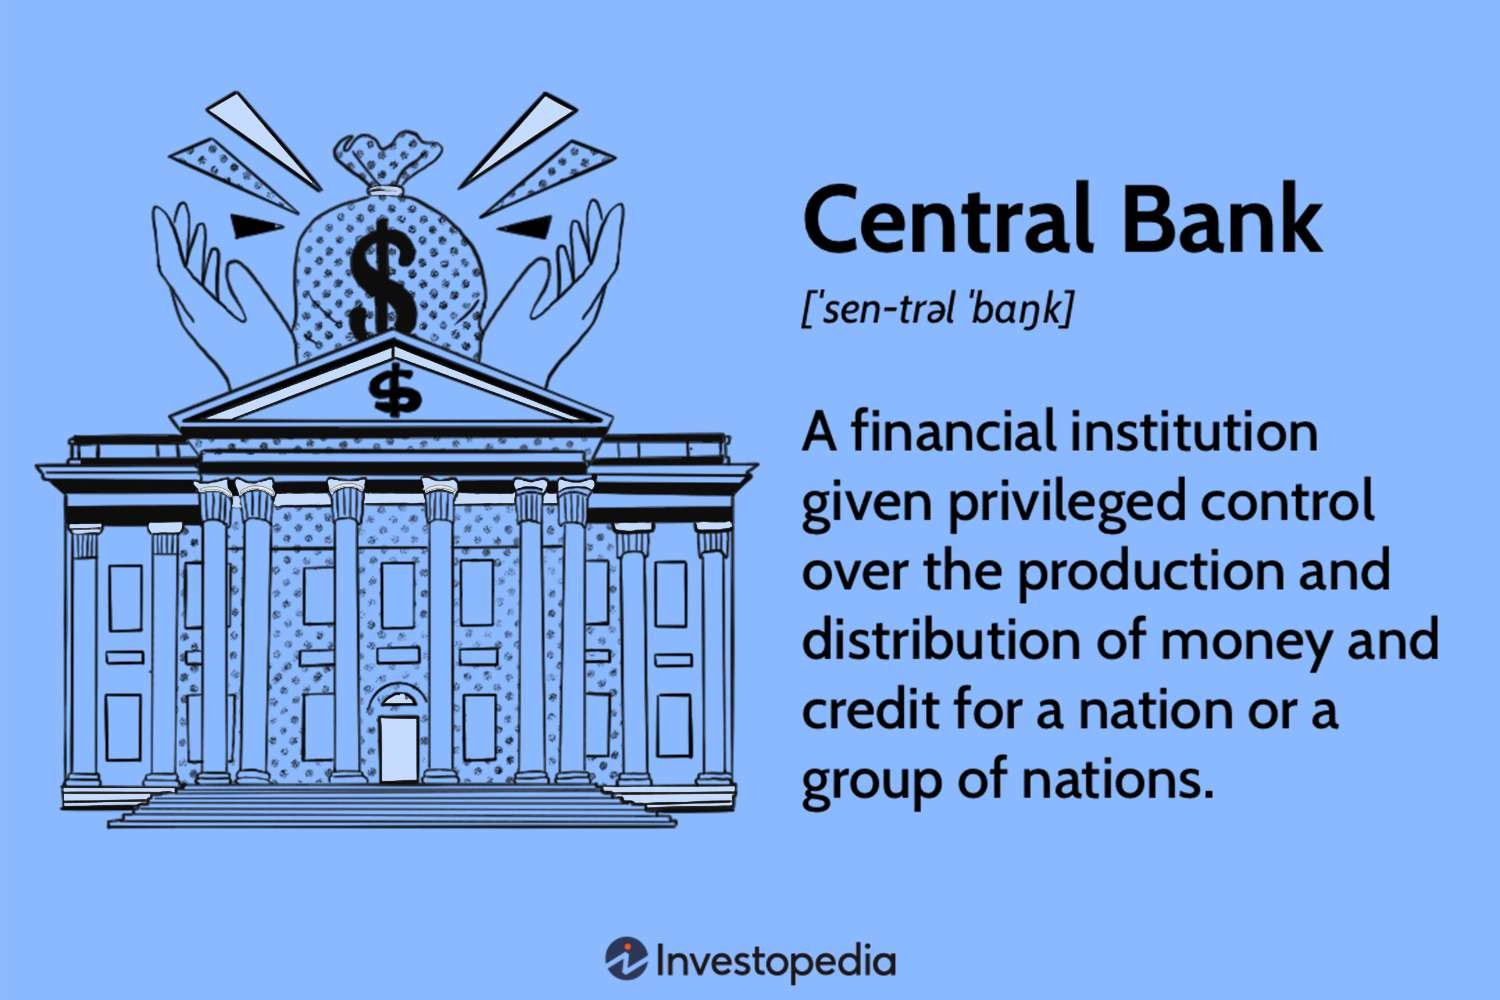
\includegraphics[scale=0.22,clip=false]{pictures/central-bank.jpg}
  \end{center}

\end{frame}

\begin{frame}\frametitle{Central banks delegate to local banks}

  Local banks use centralized (duplicated) computers to keep track of money

  \begin{center}
    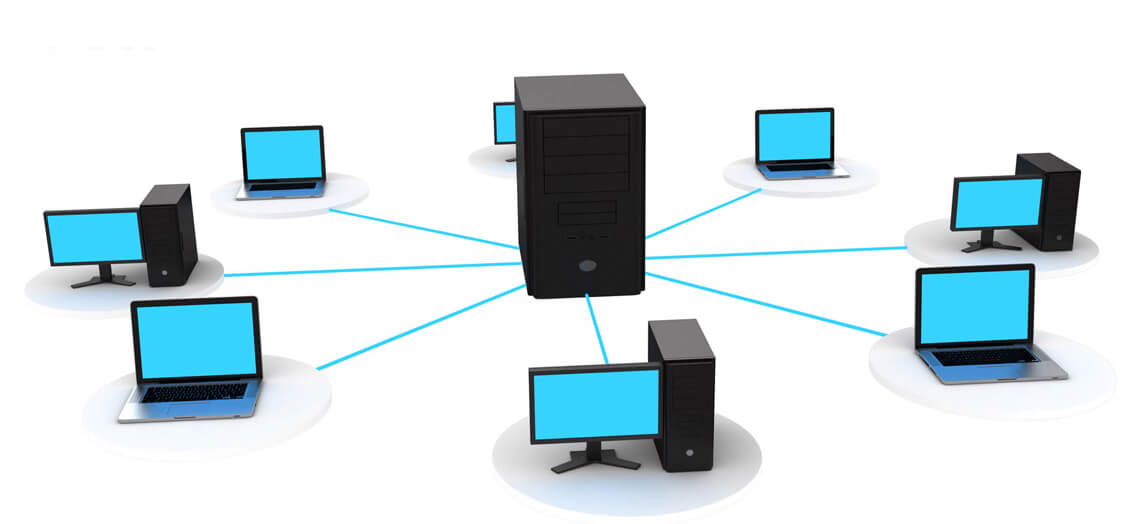
\includegraphics[scale=0.22,clip=false]{pictures/centralized-network.jpg}
  \end{center}

  \begin{greenbox}{It's all about trust}
    \begin{itemize}
    \item if a centralized computer crashes, data might get lost
    \item if data gets modified in a central computer, money could be stolen
    \end{itemize}
  \end{greenbox}
  
\end{frame}

\begin{frame}{Trust is rare in this world}

  \begin{itemize}
  \item we trust our supermarket points because they have little and limited value
  \item we trust(ed?) PayPal because we keep and exchange little money on it
  \item we trust credit card issuers up to a few thousand dollars
    because they \emph{should not} fail
    and \emph{should not} cheat (too big to fail, to big to cheat)
  \end{itemize}

\end{frame}

\begin{frame}\frametitle{Can trust arise in a trusteless world?}

  \begin{greenbox}{We want a money handling system that}
    \begin{itemize}
    \item has no central, special computer
    \item consists of many computers, all created equal
    \item if some computers fail, the network survives
    \item each computer contains all data, it does not need the others
    \item if a computer holds corrupted data, we can immediately see it
    \item the system is very unlikely to change the history of money transfers
      (no double spending)
    \end{itemize}
  \end{greenbox}

  \begin{center}
    
\includegraphics[scale=0.3,clip=false]{pictures/unicorn.jpg}
  \end{center}

\end{frame}

\begin{frame}\frametitle{Distributed network}

  \begin{center}
    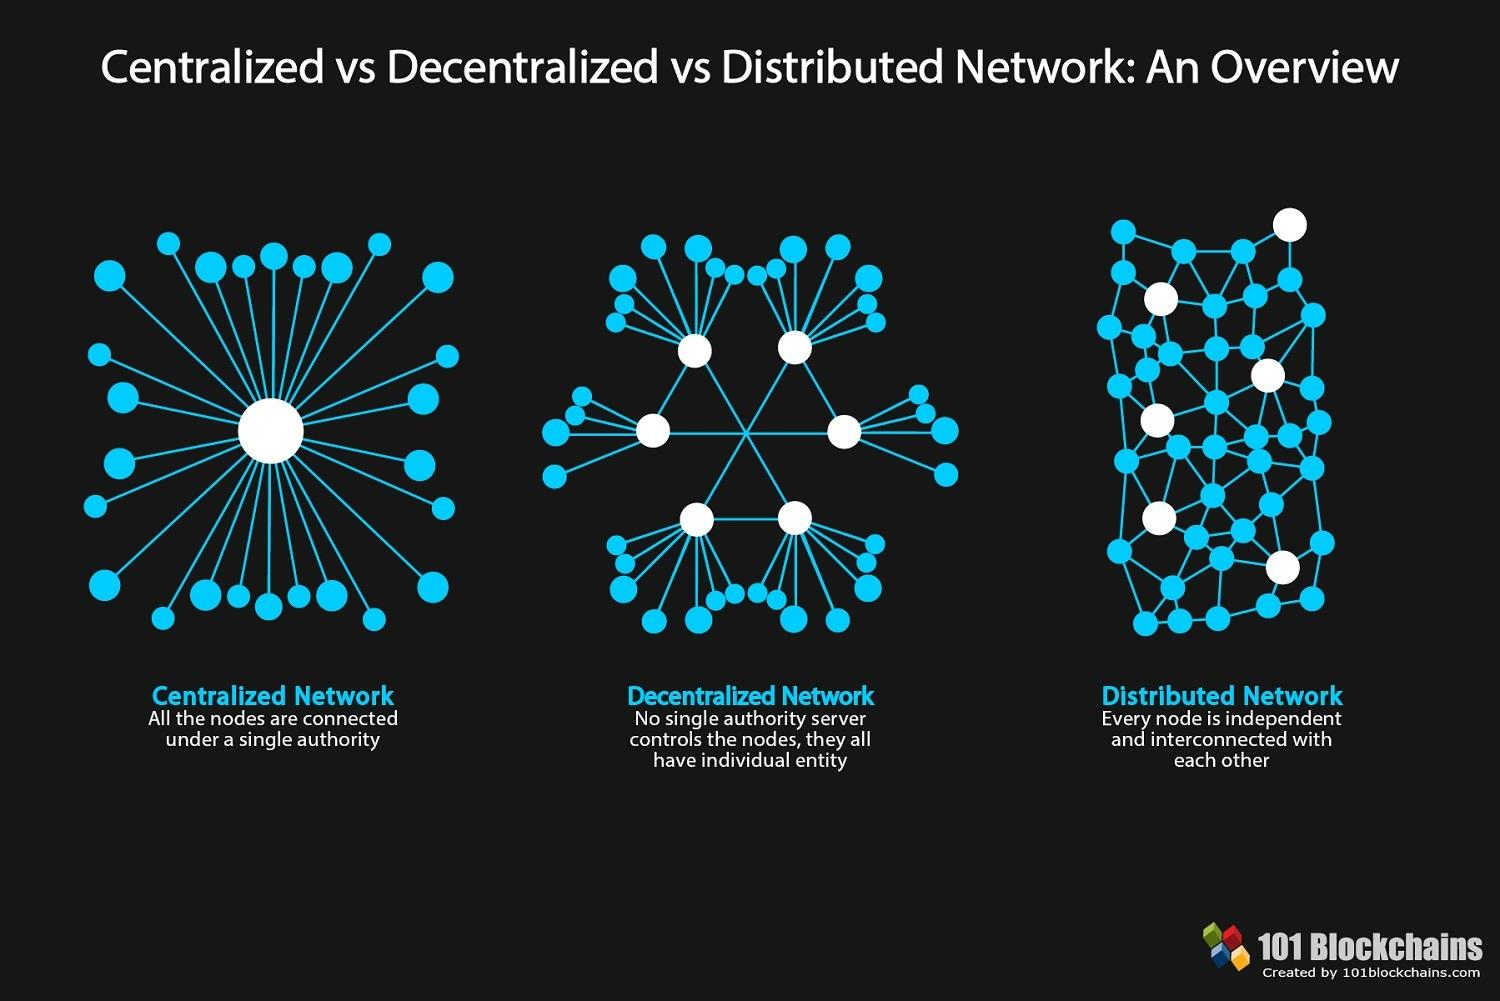
\includegraphics[scale=0.22,clip=false]{pictures/distributed.jpg}
  \end{center}

\end{frame}

\begin{frame}\frametitle{A Bit of History}

  \begin{itemize}
  \item[1991] a cryptographically secure chain of blocks (Haber \& Stornetta)
  \item[1992] proof of work (Dwork \& Naor)
  \item[2008] the sum of the two above becomes Bitcoin (Nakamoto)
  \end{itemize}

  \bigskip

  \begin{greenbox}{Why did it take so long?}
    \begin{itemize}
    \item because researchers live in isolated bubbles
    \item because the implementation was hard
    \end{itemize}
  \end{greenbox}

\end{frame}

\begin{frame}\frametitle{A Secure Chain of Blocks}

  \begin{center}
    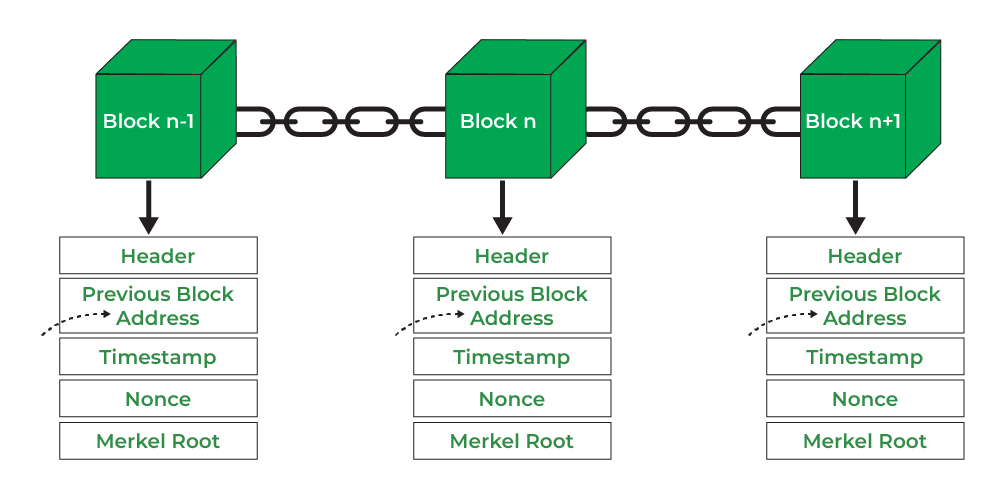
\includegraphics[scale=0.26,clip=false]{pictures/blocks.png}
  \end{center}

  If one modifies data in block $n$, then its hash changes and consequently
  blocks $n+1$, $n+2$, \ldots
  must be modified as well, because they use hashes as machine-independent backwards pointers

  \medskip

  \begin{redbox}{}
    Recomputation still possible in a few seconds for a modern computer
  \end{redbox}
  
\end{frame}

\begin{frame}\frametitle{Proof of Work}

  \begin{redbox}{}
    Cynthia Dwork and Noni Naor (1992). “Pricing via Processing, Or, Combatting Junk Mail, Advances in Cryptology”. CRYPTO’92: Lecture Notes in Computer Science No. 740. Springer: 139–147.
  \end{redbox}

  \bigskip

  \begin{tabular}{ccc}
    text of email & hashing & \\
    recipient address & $\Rightarrow$ & $\mathtt{\underbrace{0000000}43f5e6bc00d56984\ldots5974edf}$\\
    date of the email && \\
    numerical nonce &&
  \end{tabular}

  \bigskip

  The email client will accept the email only if the hash starts with at least seven (or more) zeros

  \bigskip

  The sender needs to try and retry the hashing by changing the nonce, until it finds a good hash that will be accepted

  \bigskip

  This takes time and consumes energy: it makes spam expensive

\end{frame}

\begin{frame}\frametitle{Bitcoin = Secure chain of blocks + Proof of work}

  \begin{center}
    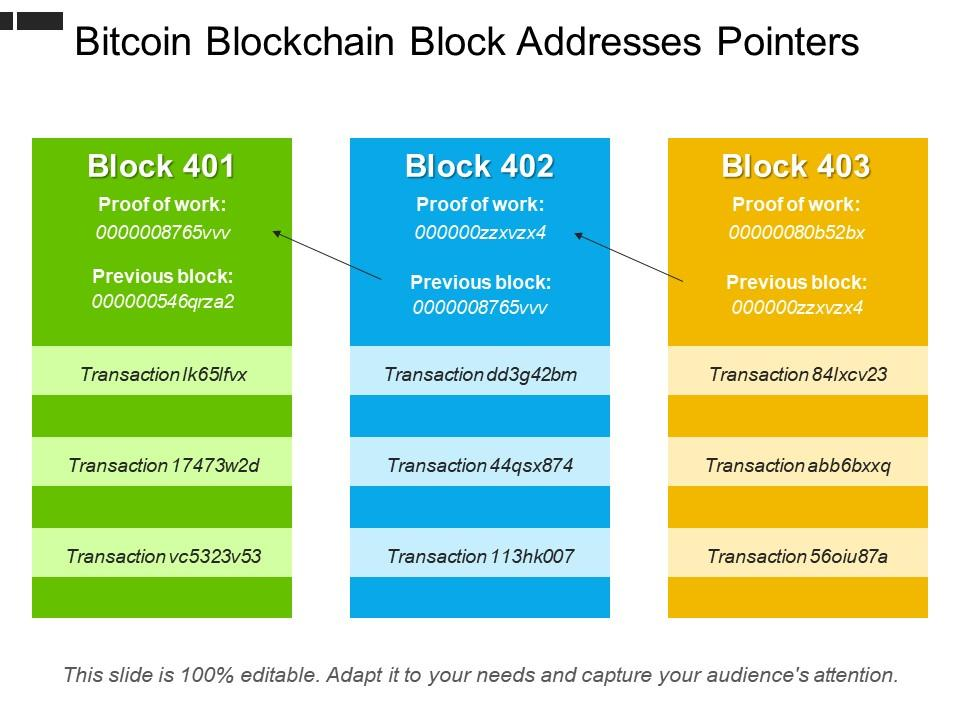
\includegraphics[scale=0.28,clip=false]{pictures/blocks-pow.jpg}
  \end{center}

  \smallskip

  If one modifies data in block $n$, then its hash changes and consequently
  blocks $n+1$, $n+2$, \ldots
  must be modified as well, but this requires to recompute the proof of work
  (a correct nonce for each recomputed block)

  \smallskip

  \begin{redbox}{}
    Recomputation could take centuries even on very fast computer
  \end{redbox}
\end{frame}

\begin{frame}\frametitle{Consensus rules}

  \begin{itemize}
  \item timestamps can only increase
  \item remuneration for block creation is computed according to the right formula
  \item the (ordered) execution of the transactions in the blocks do not fail
  \item starting from the state whose Merkle root is in block $n$ and executing
    the transactions in block $n+1$ (in their order), one obtain a state whose Merkle root is
    in block $n+1$
  \item \ldots
  \end{itemize}
\end{frame}

\begin{frame}\frametitle{Proof-of-work (PoW)}

  \begin{greenbox}{Add the following consensus rule}
    The hash of the blocks is smaller than
    a value called $\mathit{difficulty}$
  \end{greenbox}

  \bigskip

  \begin{greenbox}{Each miner does some work}
    \begin{enumerate}
    \item builds a new block
    \item sets the nonce field of its header to a random value
    \item computes the hash $h$ of the header
    \item if $h < \mathit{difficulty}$ it stops
    \item otherwise, it goes back to step~2
    \end{enumerate}
  \end{greenbox}

  \bigskip

  \begin{itemize}
  \item the PoW is the fact that the hash of the resulting block is small
  \item the time to solve this puzzle is inversely proportional to $\mathit{difficulty}$
  \item the algorithm can be easily run in parallel
  \end{itemize}

\end{frame}

\begin{frame}\frametitle{The blockchain grows}

  \begin{itemize}
  \item each miner creates a new block on top of the main history
  \item at the same time, each miner receives alternative new blocks from its peers
    \begin{itemize}
    \item blocks whose parent is the top of the main history, or
    \item whose parent is another block of the blockchain (fork), or
    \item whose parent is unknown to the miner (orphan block)
    \end{itemize}
  \item in case of fork, the main history is the longest one (actually: the most powerful one), but miners keep all histories,
    in case they might become the new main history in the future
  \item the blockchain is actually a tree, not a list
  \end{itemize}

  \[
  \mathit{power}(\mathit{chain})=\sum_{\mathit{block}\in\mathit{chain}}\frac{2^{8\cdot 32}}{\mathit{hash}(\mathit{block})+1}
  \]
\end{frame}

\begin{frame}\frametitle{Fork: all miners start with the same vision}

  \begin{center}
    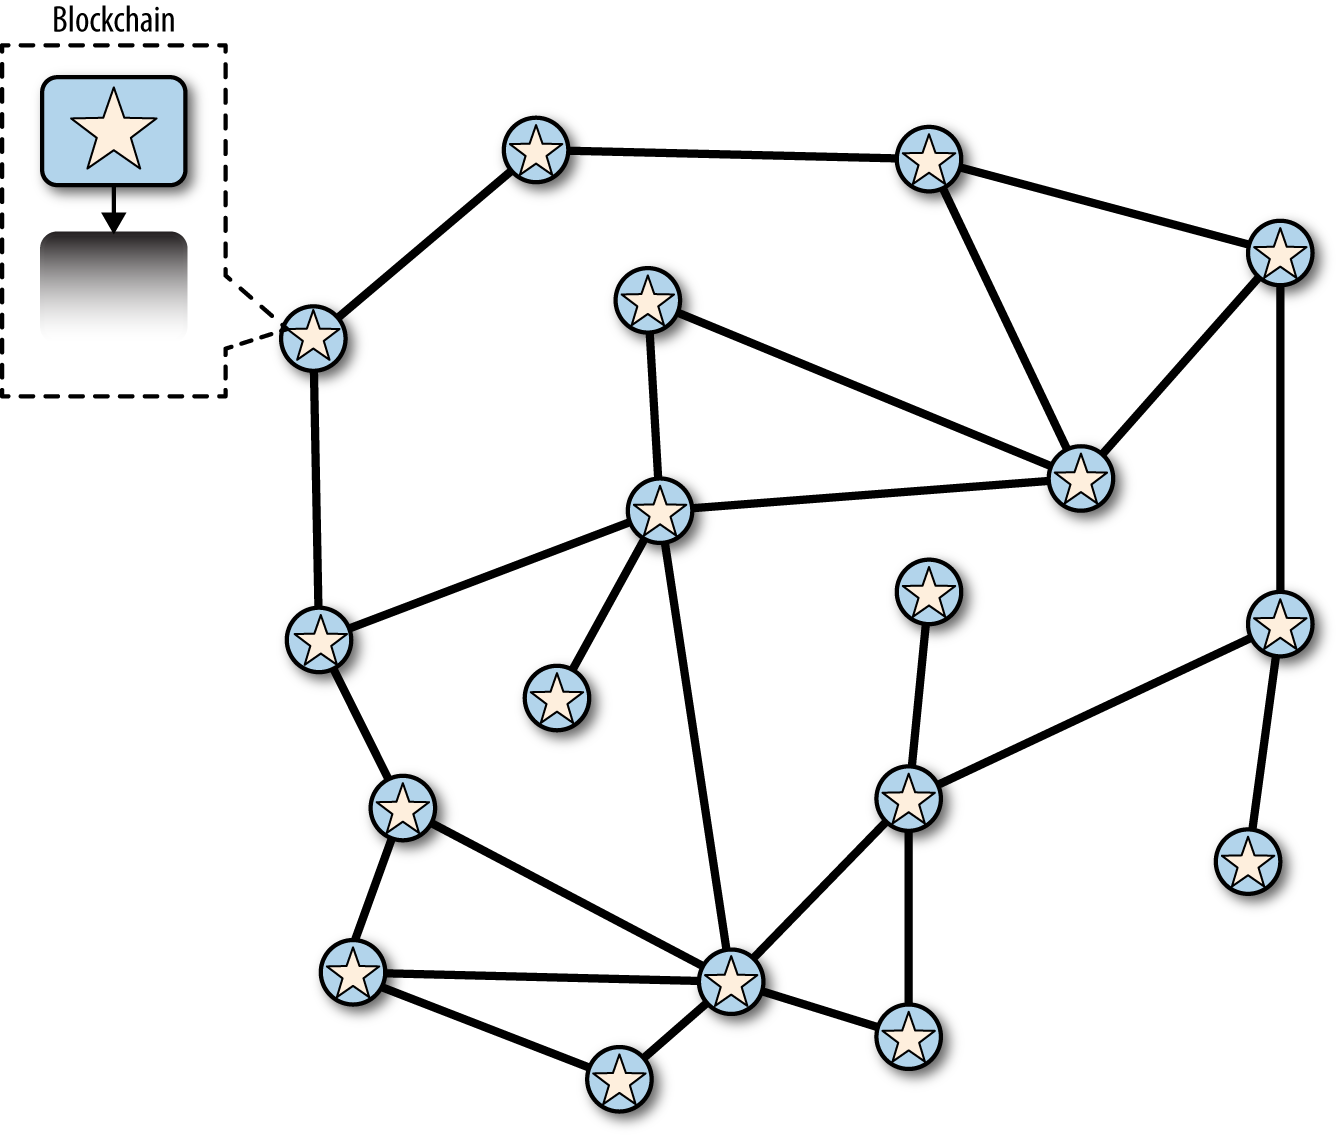
\includegraphics[scale=0.8,clip=false]{pictures/mbc2_1002.png}
  \end{center}

\end{frame}

\begin{frame}\frametitle{Fork: two miners expand the blockchain simultaneously}

  \begin{center}
    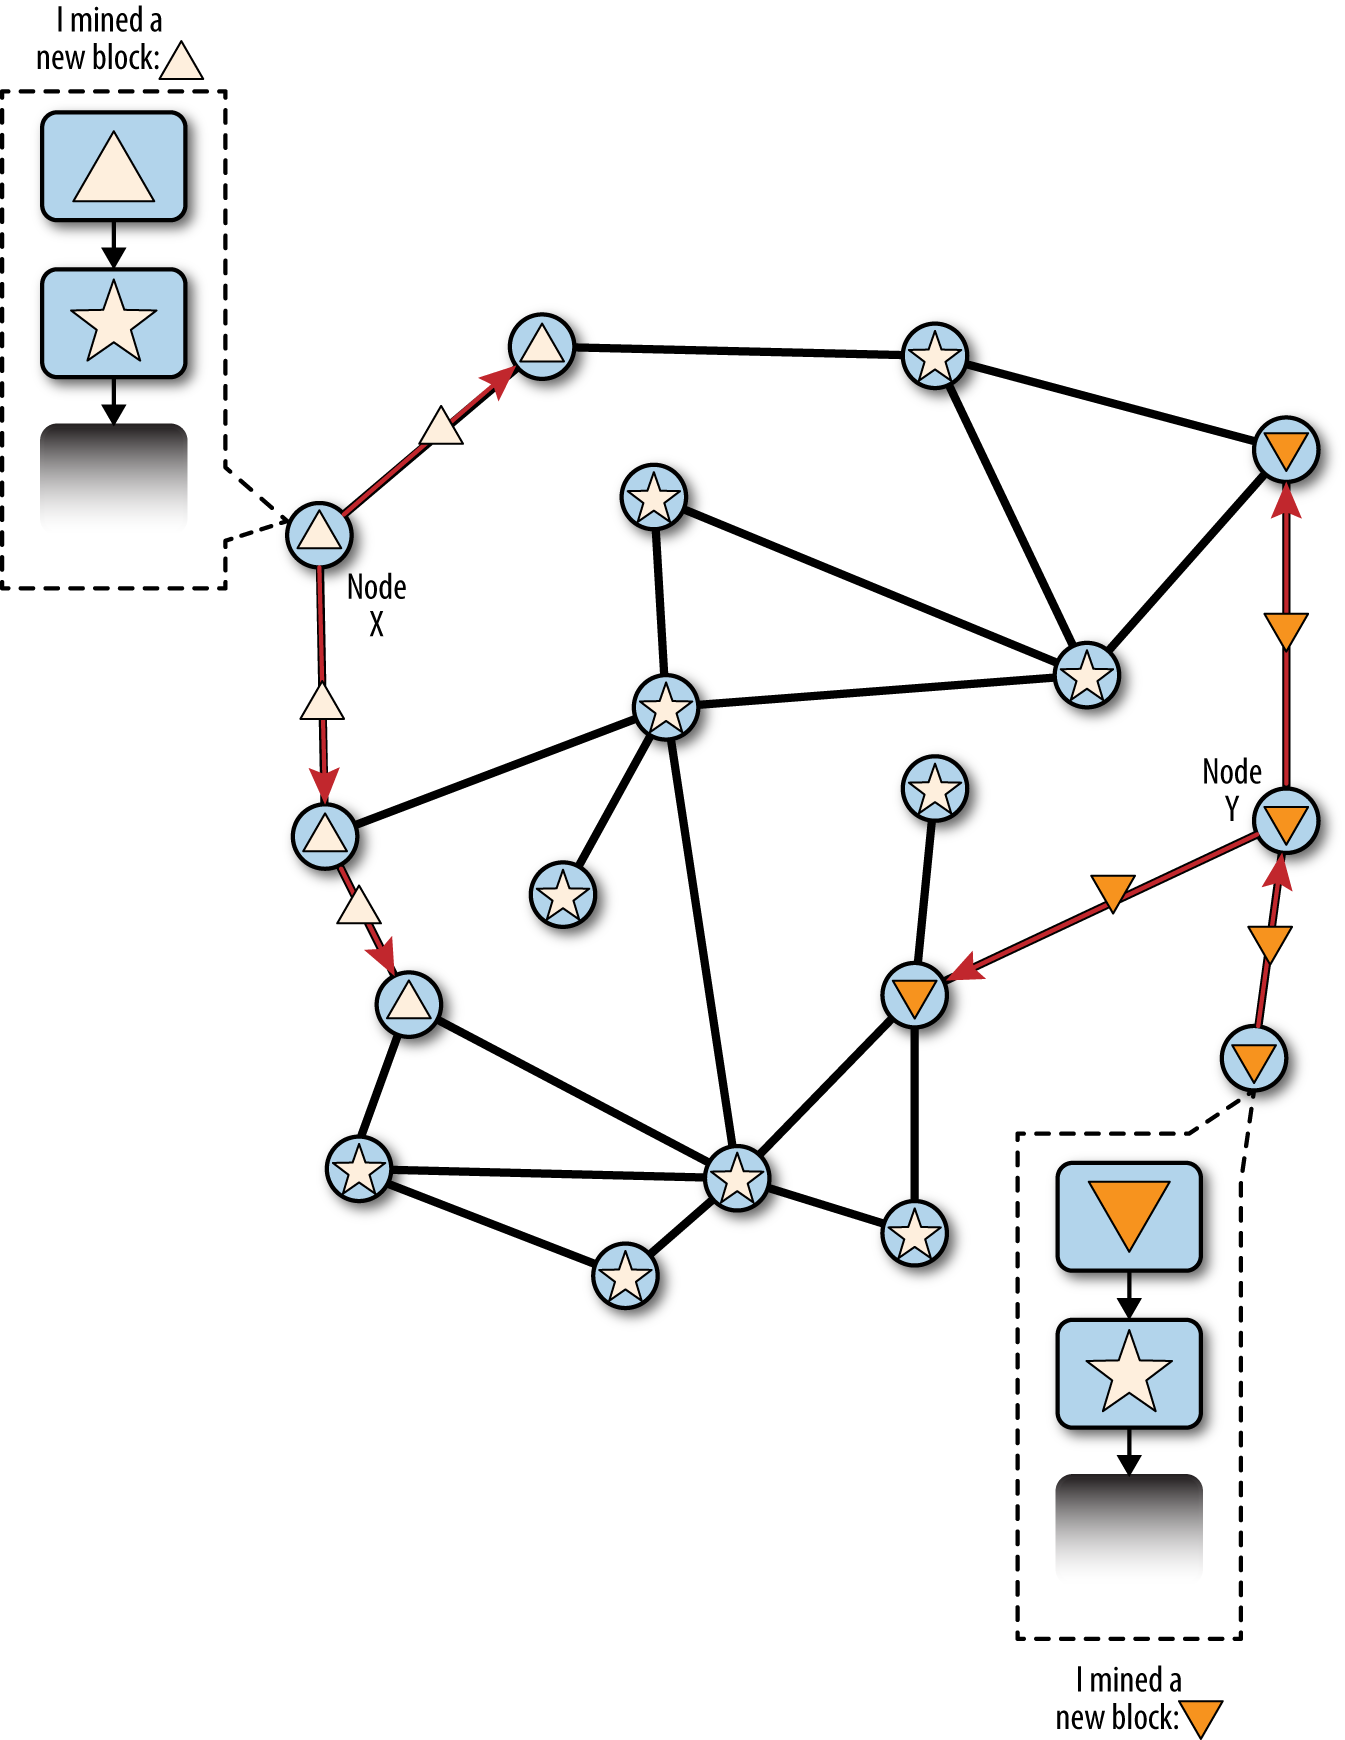
\includegraphics[scale=0.53,clip=false]{pictures/mbc2_1003.png}
  \end{center}

\end{frame}

\begin{frame}\frametitle{Fork: the network is split}

  \begin{center}
    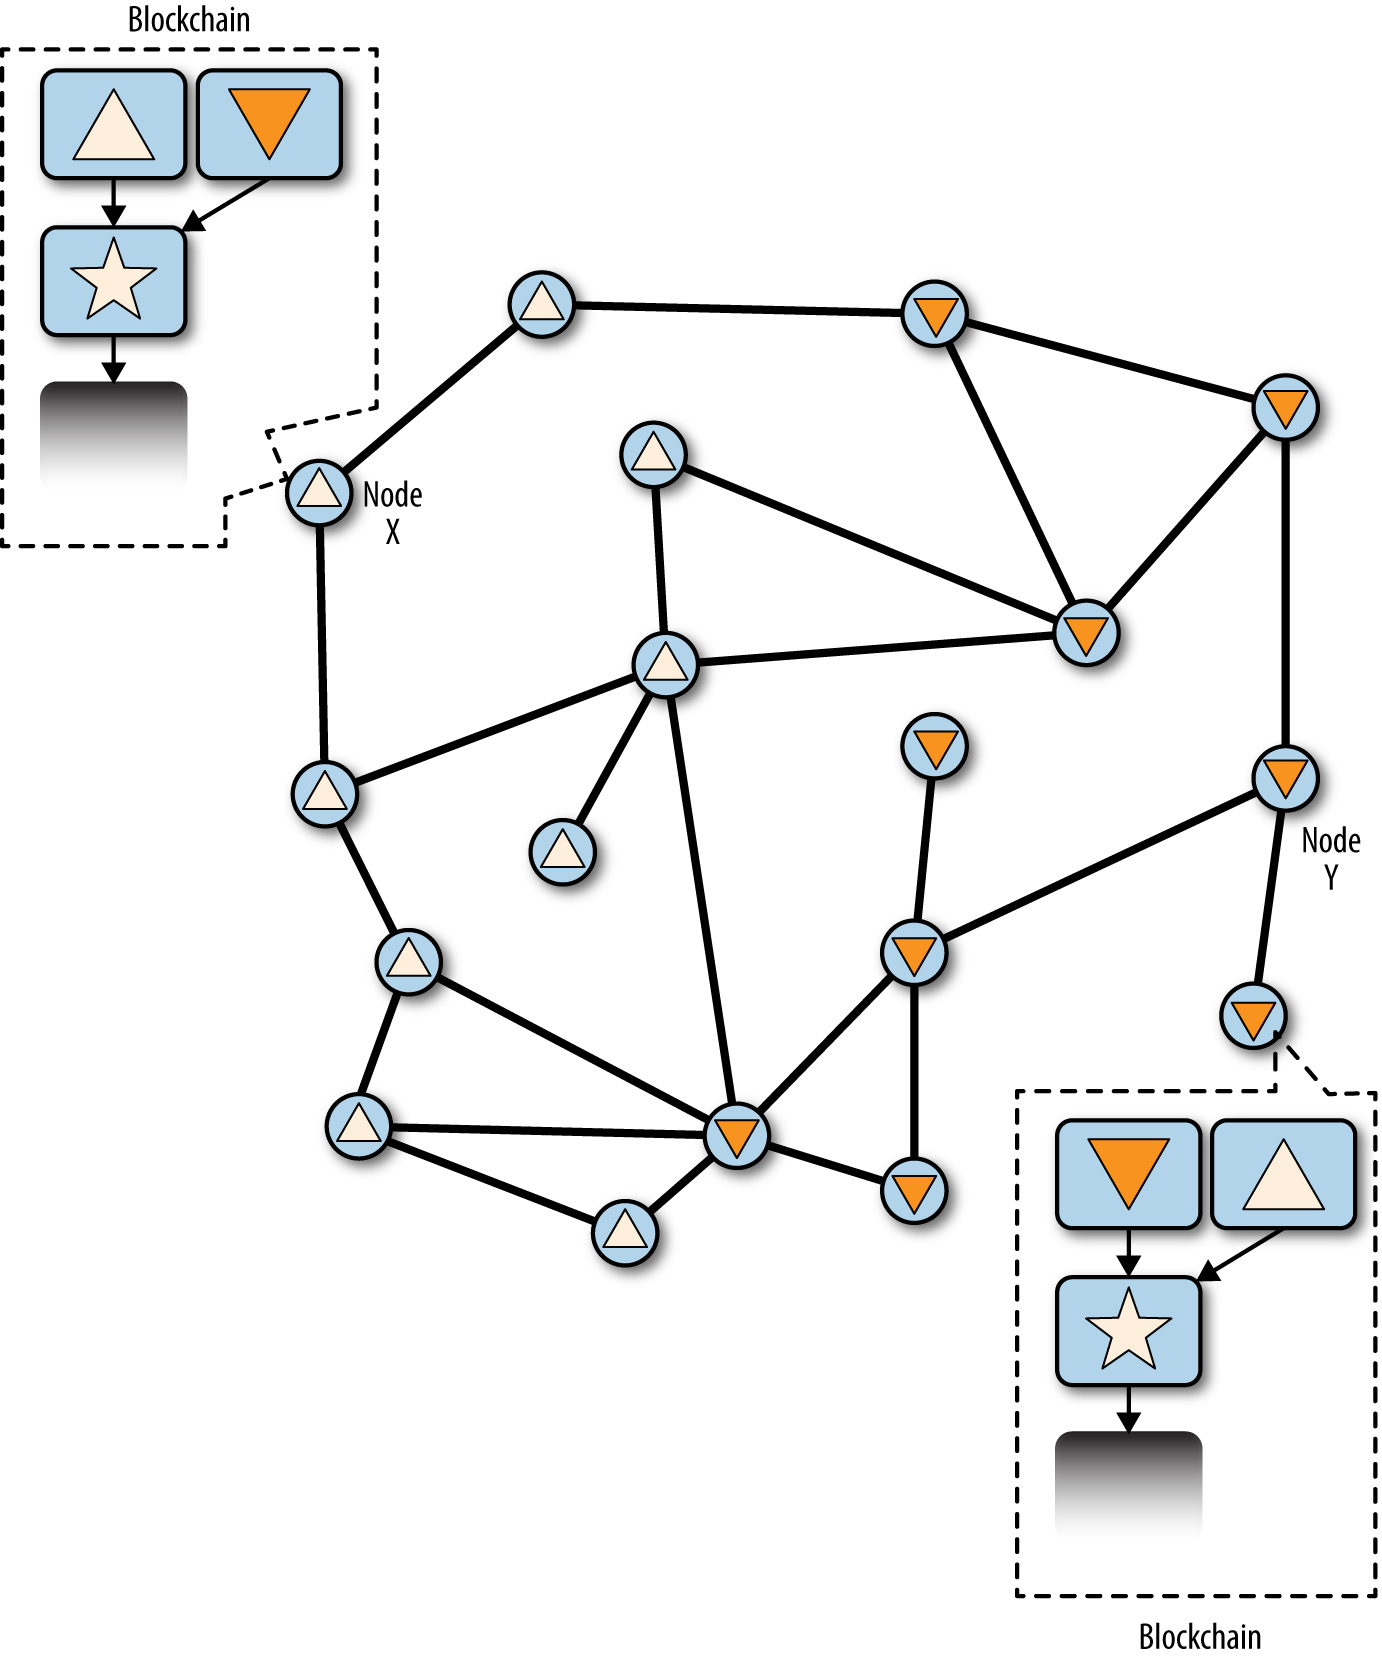
\includegraphics[scale=0.56,clip=false]{pictures/mbc2_1004.png}
  \end{center}

\end{frame}

\begin{frame}\frametitle{Fork: either chain is expanded further}

  \begin{center}
    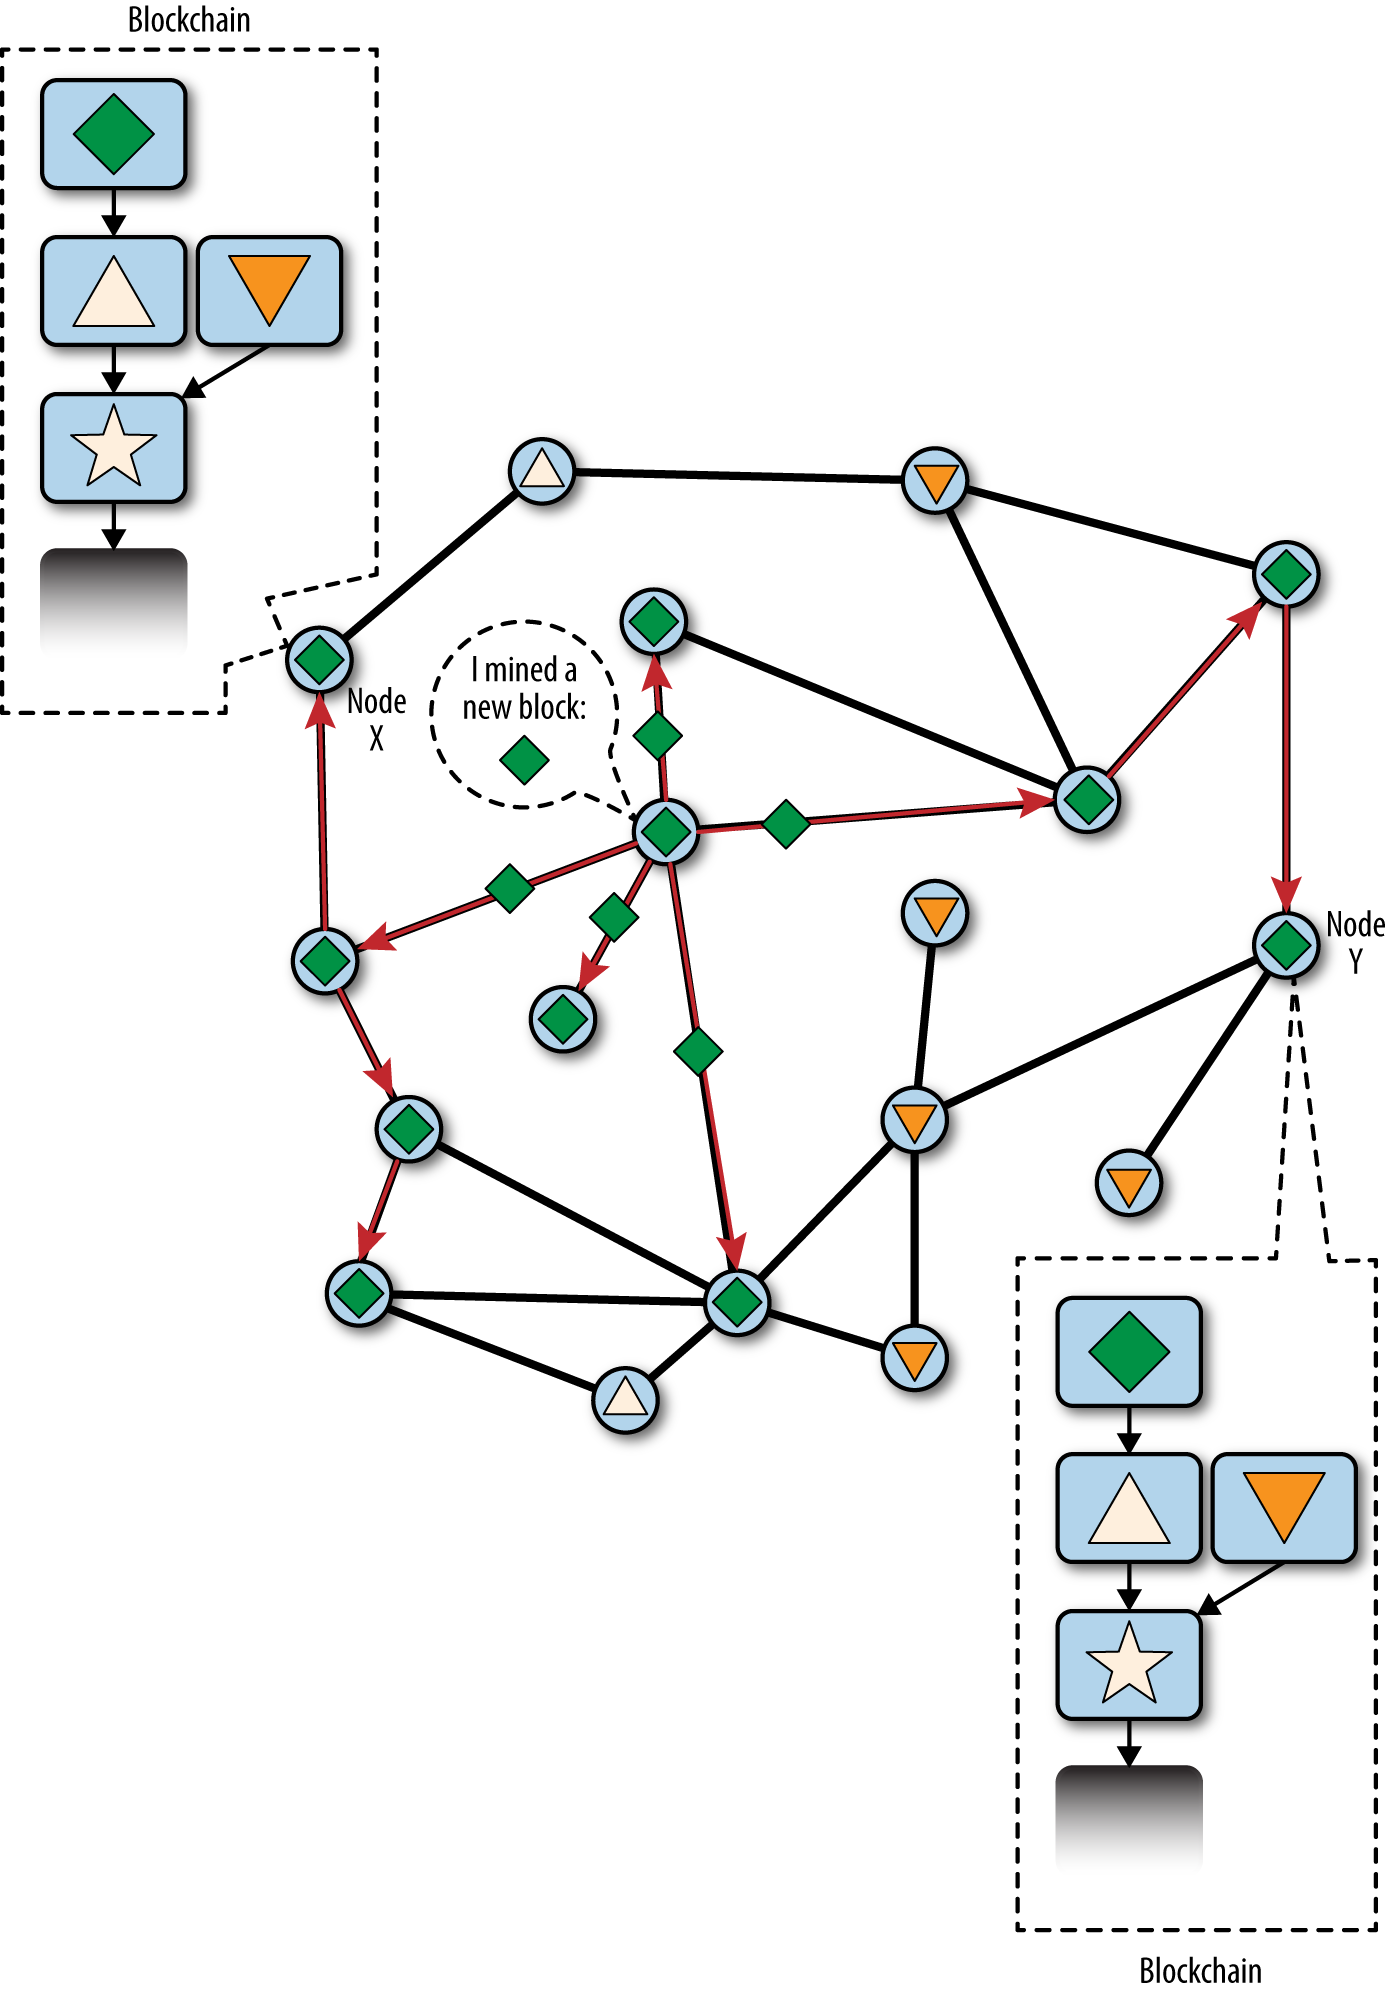
\includegraphics[scale=0.47,clip=false]{pictures/mbc2_1005.png}
  \end{center}

\end{frame}

\begin{frame}\frametitle{Fork: the network reconverges}

  \begin{center}
    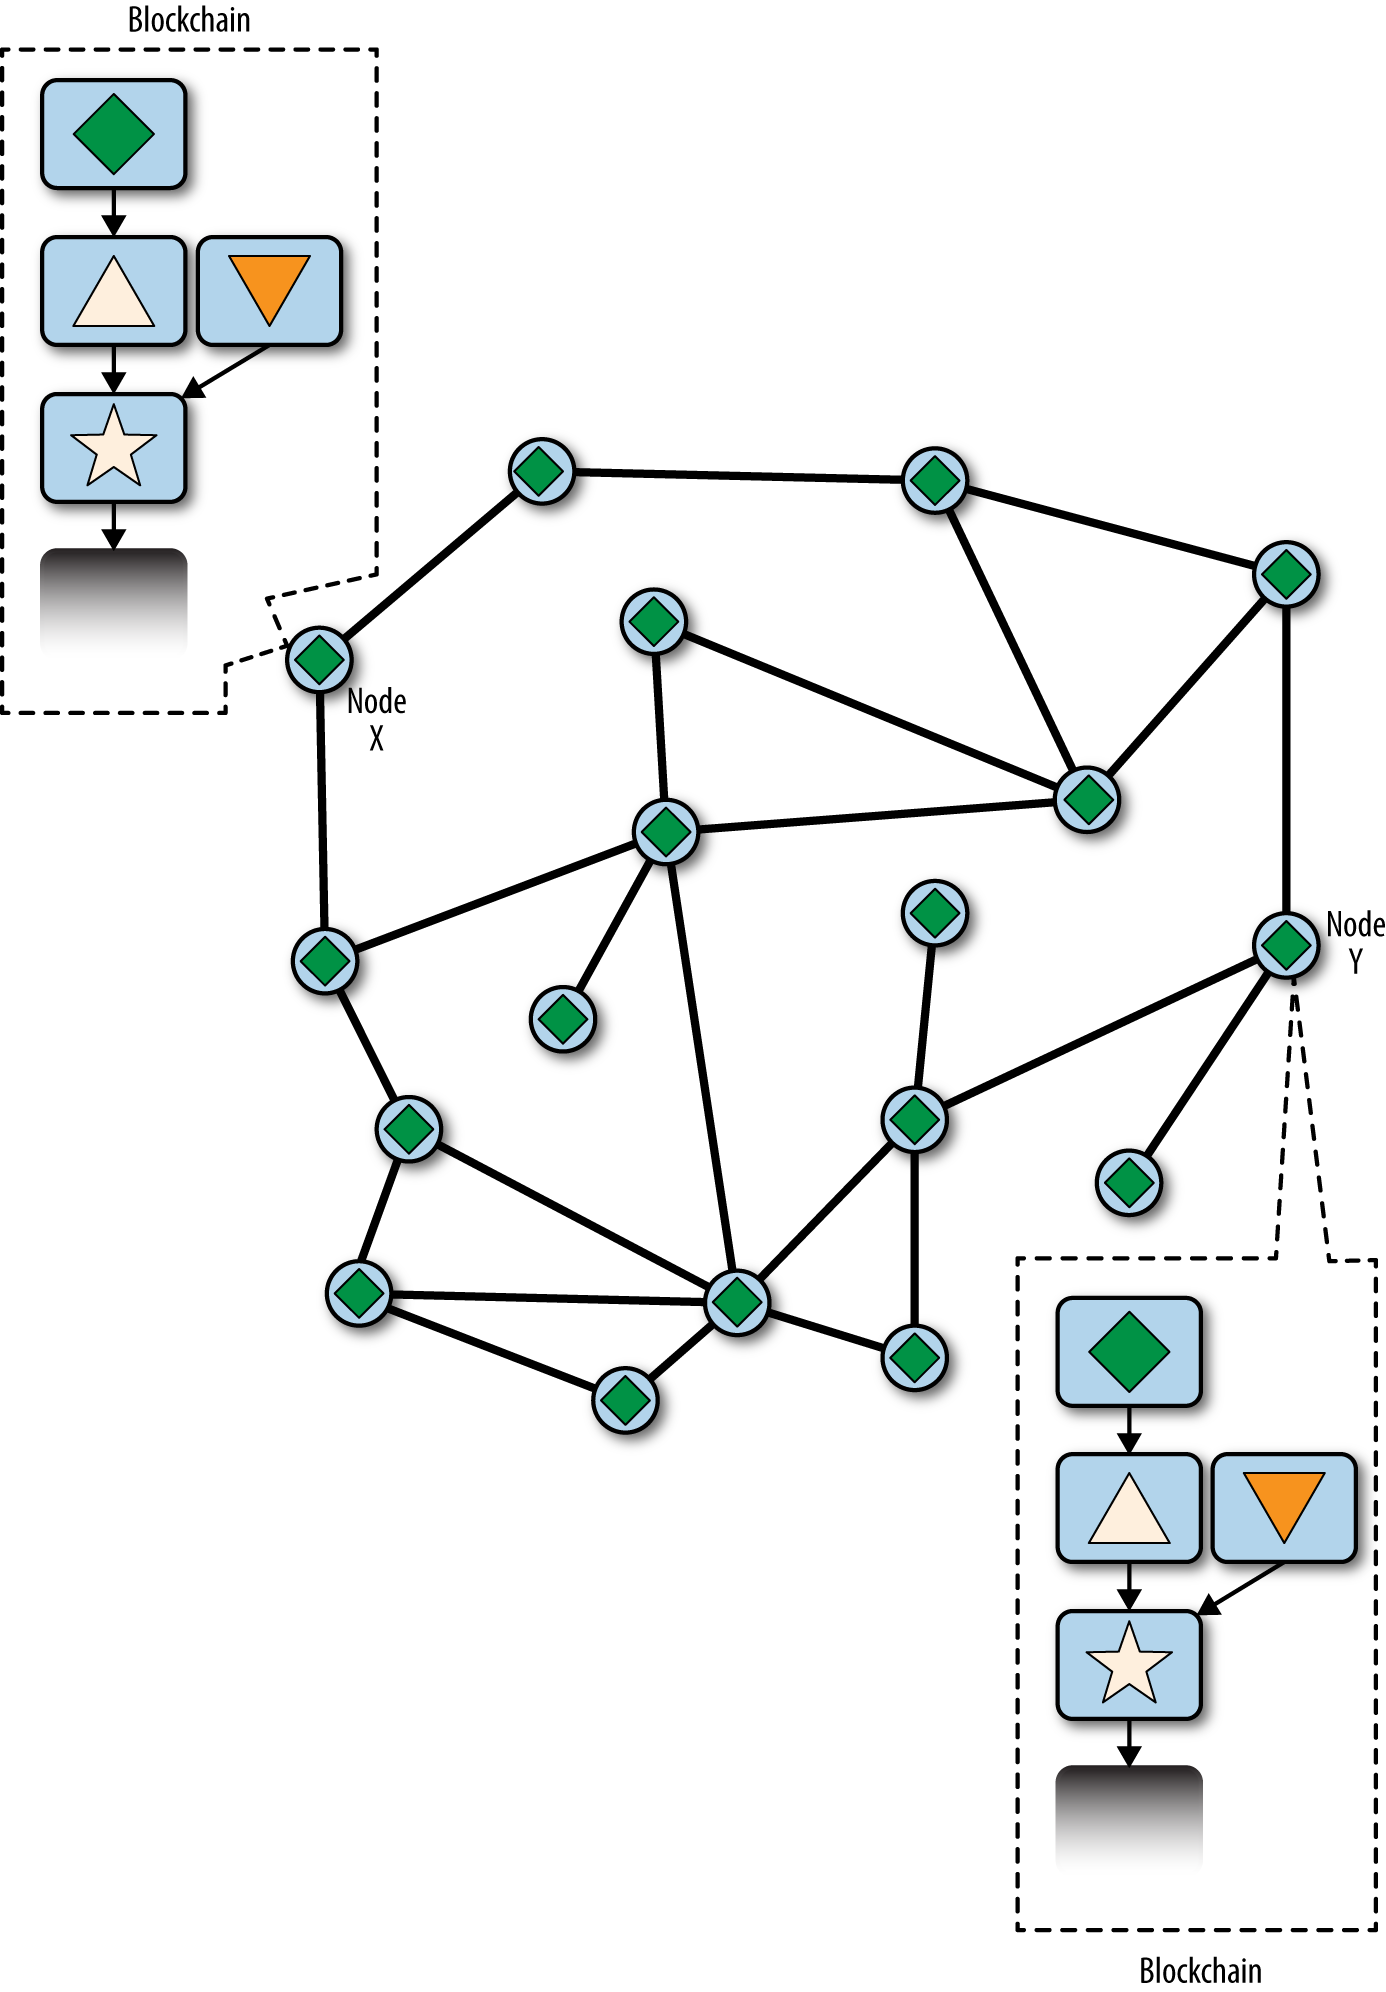
\includegraphics[scale=0.47,clip=false]{pictures/mbc2_1006.png}
  \end{center}

\end{frame}

\begin{frame}\frametitle{How to kill a dictator}

  \begin{greenbox}{Without proof of work}
    A single node can dictate the history of the blockchain
    if it is faster than \emph{each} other node
  \end{greenbox}

  \pause
  \bigskip
  \bigskip

  \begin{greenbox}{With proof of work}
    A single node can dictate the history of the blockchain
    if it is faster than \emph{the sum of all} other nodes
  \end{greenbox}

\end{frame}

\begin{frame}\frametitle{The magic behind the proof of work}

  \begin{greenbox}{}
    It makes expensive the production of new blocks, in time and cost (electricity)
    \begin{itemize}
    \item who produces invalid blocks sees its blocks rejected by peers and wastes resources
    \item a single node cannot dictate the history easily, since it must fight against
      the hashing power of all other nodes together
    \item forks become unlikely, since the probability of two nodes finding a new block at the same time is small
    \end{itemize}
  \end{greenbox}

\end{frame}

\begin{frame}\frametitle{Evolution of the miners}

  \begin{center}
    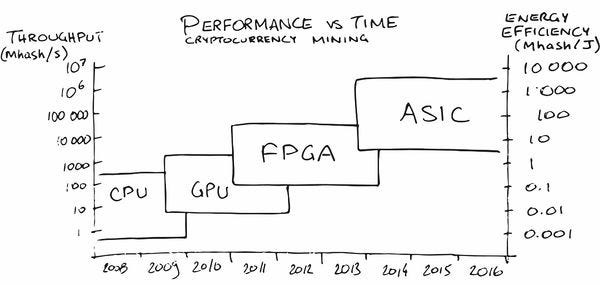
\includegraphics[scale=0.55,clip=false]{pictures/mining-hardware.jpg}
  \end{center}

\end{frame}

\begin{frame}\frametitle{Difficulty over time}

  \begin{center}
    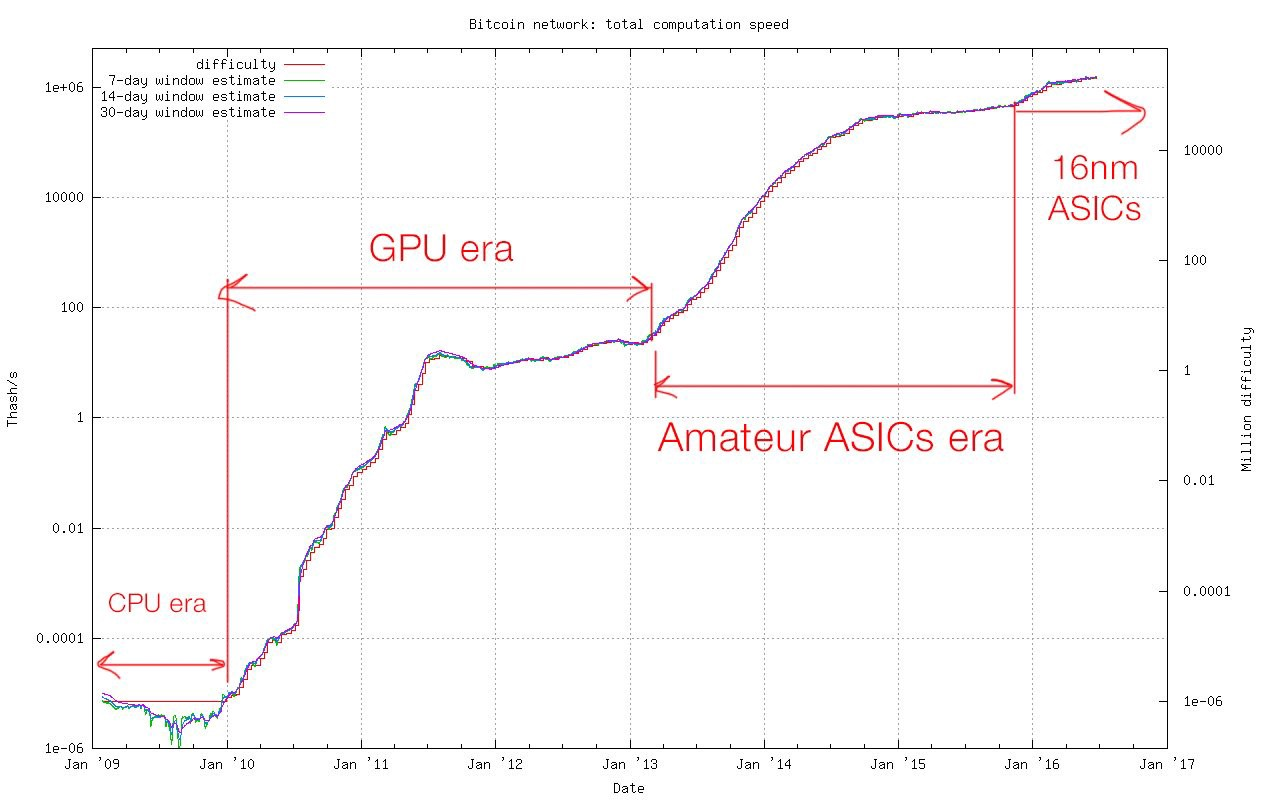
\includegraphics[width=\textwidth,clip=false]{pictures/difficulty.jpg}
  \end{center}

\end{frame}

\begin{frame}\frametitle{PoW costs electricity}

  \begin{greenbox}{2019}
    \begin{center}
      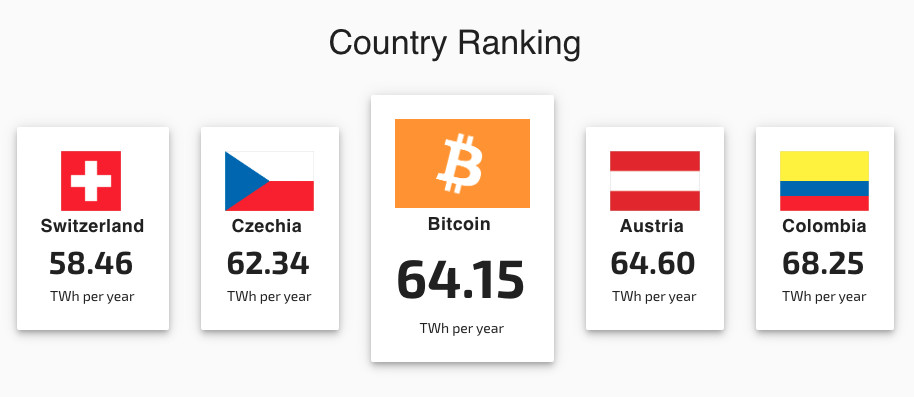
\includegraphics[scale=0.17,clip=false]{pictures/bitcoin-consumption.jpg}
      
\includegraphics[scale=0.14,clip=false]{pictures/greta.jpg}
    \end{center}
  \end{greenbox}
    
\end{frame}

\begin{frame}\frametitle{Blockhains are used for cryptocurrencies}

  \begin{center}
    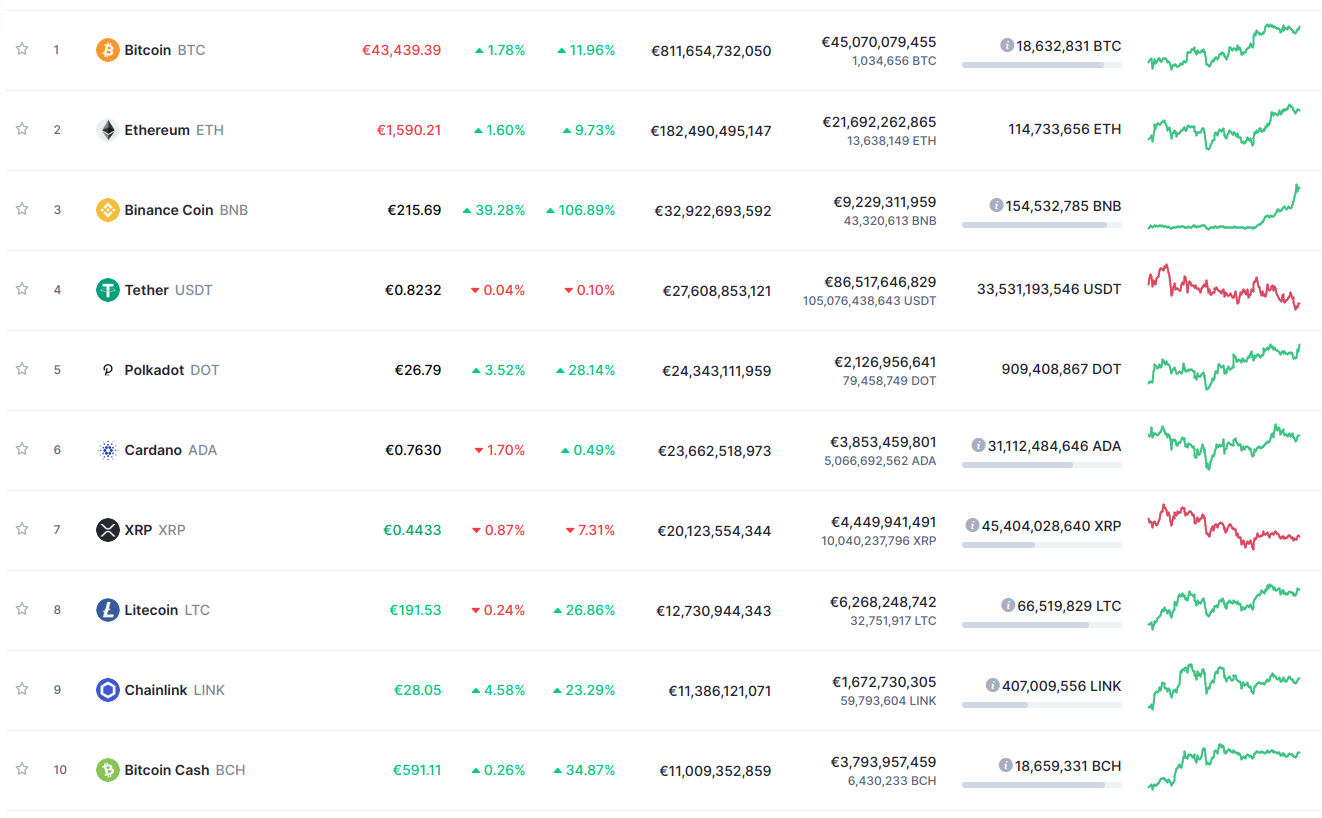
\includegraphics[scale=0.258,clip=false]{pictures/market.png}
  \end{center}

\end{frame}

\begin{frame}\frametitle{Blockhains are used for notarization}

  \begin{center}
    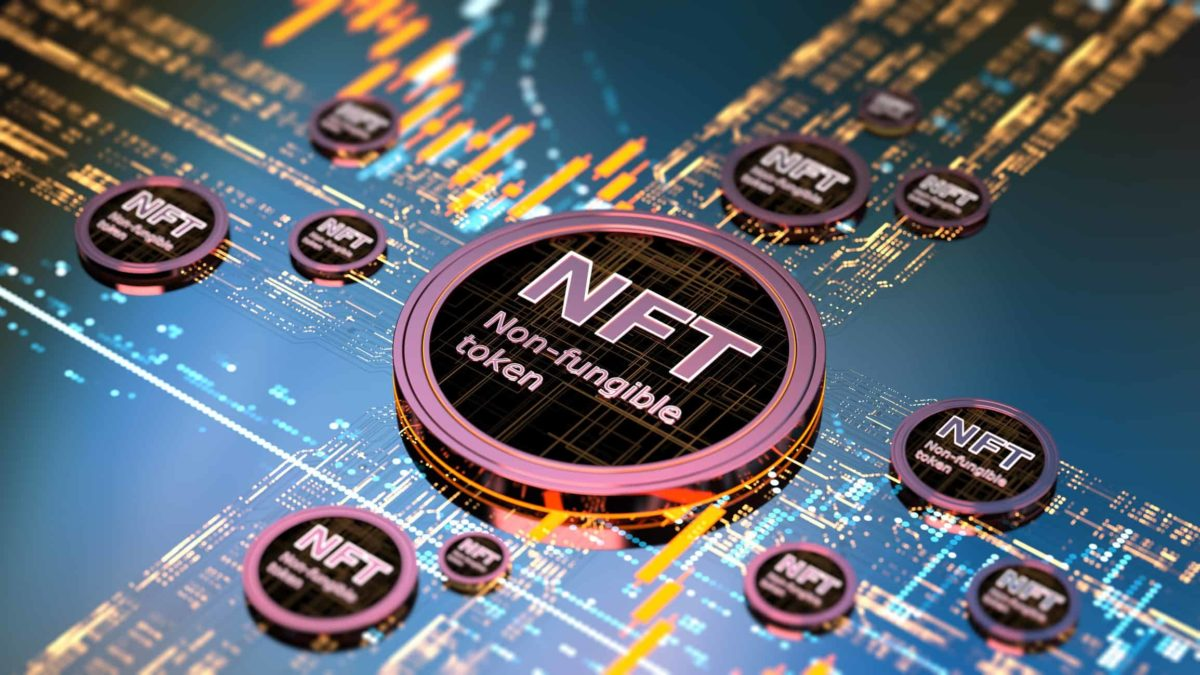
\includegraphics[scale=0.258,clip=false]{pictures/nft.jpg}
  \end{center}

\end{frame}

\begin{frame}\frametitle{Blockhains are used for ransom}

  \begin{center}
    
\includegraphics[scale=0.7, clip=false]{pictures/ransom.jpg}
  \end{center}

  \begin{redbox}{}
    Send one bitcoin to this account if you want your data decrypted!
  \end{redbox}

\end{frame}

\begin{frame}\frametitle{Blockhains are used to circumvent international rules or bans}

  \begin{center}
    
\includegraphics[scale=1, clip=false]{pictures/send-money.jpg}
  \end{center}

\end{frame}

\begin{frame}\frametitle{Is all this worth its energy consumption and pollution?}

  \begin{center}
    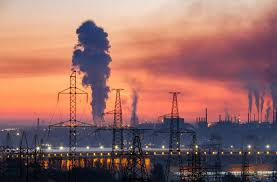
\includegraphics[scale=1, clip=false]{pictures/pollution.jpg}
  \end{center}

\end{frame}

\begin{frame}
  \frametitle{Can blockchain work without wasting energy?}

  \begin{center}
    Who decides the next block?
  \end{center}

  \bigskip

  \begin{greenbox}{}
    \begin{itemize}
    \item proof of work [PoW] (who works harder)
    \item proof of stake [PoS] (who commits more money)
    \item proof of space [PoSp] (who commits more disk space)
    \item proof of authority [PoA] (who has more authority)
    \item \ldots
    \end{itemize}
  \end{greenbox}

  \bigskip

  \begin{greenbox}{PoS is a variant of Practical Byzantine Fault Tolerance (BFT)}
    Miguel Castro and Barbara Liskov.
    \emph{Practical Byzantine Fault Tolerance and Proactive Recovery}.
    ACM Trans.\ Comput.\ Syst., 20(4):398–461, November 2002
  \end{greenbox}

\end{frame}

\begin{frame}\frametitle{Tendermint (now Ignite): \url{ignite.com}}

  \begin{greenbox}{Jae Kwon. \emph{Tendermint: Consensus without Mining}, 2014.\\
    \url{https://www.weusecoins.com/assets/pdf/library/Tendermint\ Consensus\ without\ Mining.pdf}}
    \begin{itemize}
    \item only a set $V$ of \emph{validators} decides the next block
    \item to become validator, one must stake a large amount of money
    \item if a validator produces illegal blocks or misbehaves, the forzen money will be reduced
    \end{itemize}
  \end{greenbox}

  \smallskip

  \begin{center}
    The idea is that who has money has more interest in the health of the blockchain
  \end{center}

  \smallskip

  \begin{center}
    Low energy consumption, but this is not really decentralized!
  \end{center}

\end{frame}

\begin{frame}\frametitle{Tendermint's protocol}

  \begin{greenbox}{}
    \begin{itemize}
    \item a dynamic set $V$ of validators decides the next block
    \item $V$ might be different for each block
      \begin{itemize}
      \item but deterministically computed from the previous history
      \end{itemize}
    \item at each height $H$, each validator $v\in V$:
      \begin{enumerate}
      \item identifies (deterministically) a validator $m\in V$ that
        is expected to aggregate some transactions and \alert{propose} a next block $b$
      \item if it considers $b$ valid, it \alert{pre-votes} $b$
      \item counts how many validators pre-vote $b$
      \item if it counts at least $\frac{2}{3}$ pre-votes, it \alert{pre-commits} $b$
      \item counts how many validators pre-commit $b$
      \item if it counts at least $\frac{2}{3}$ pre-commits, it \alert{commits} $b$ and increases $H$
      \item goes back to step~1
      \end{enumerate}
    \end{itemize}
  \end{greenbox}

  \smallskip

  \begin{center}
    Tendermint is BFT. If step~1 is based on stakes, then it is PoS
  \end{center}

\end{frame}

\begin{frame}\frametitle{Tendermint's polka}

  \begin{center}
    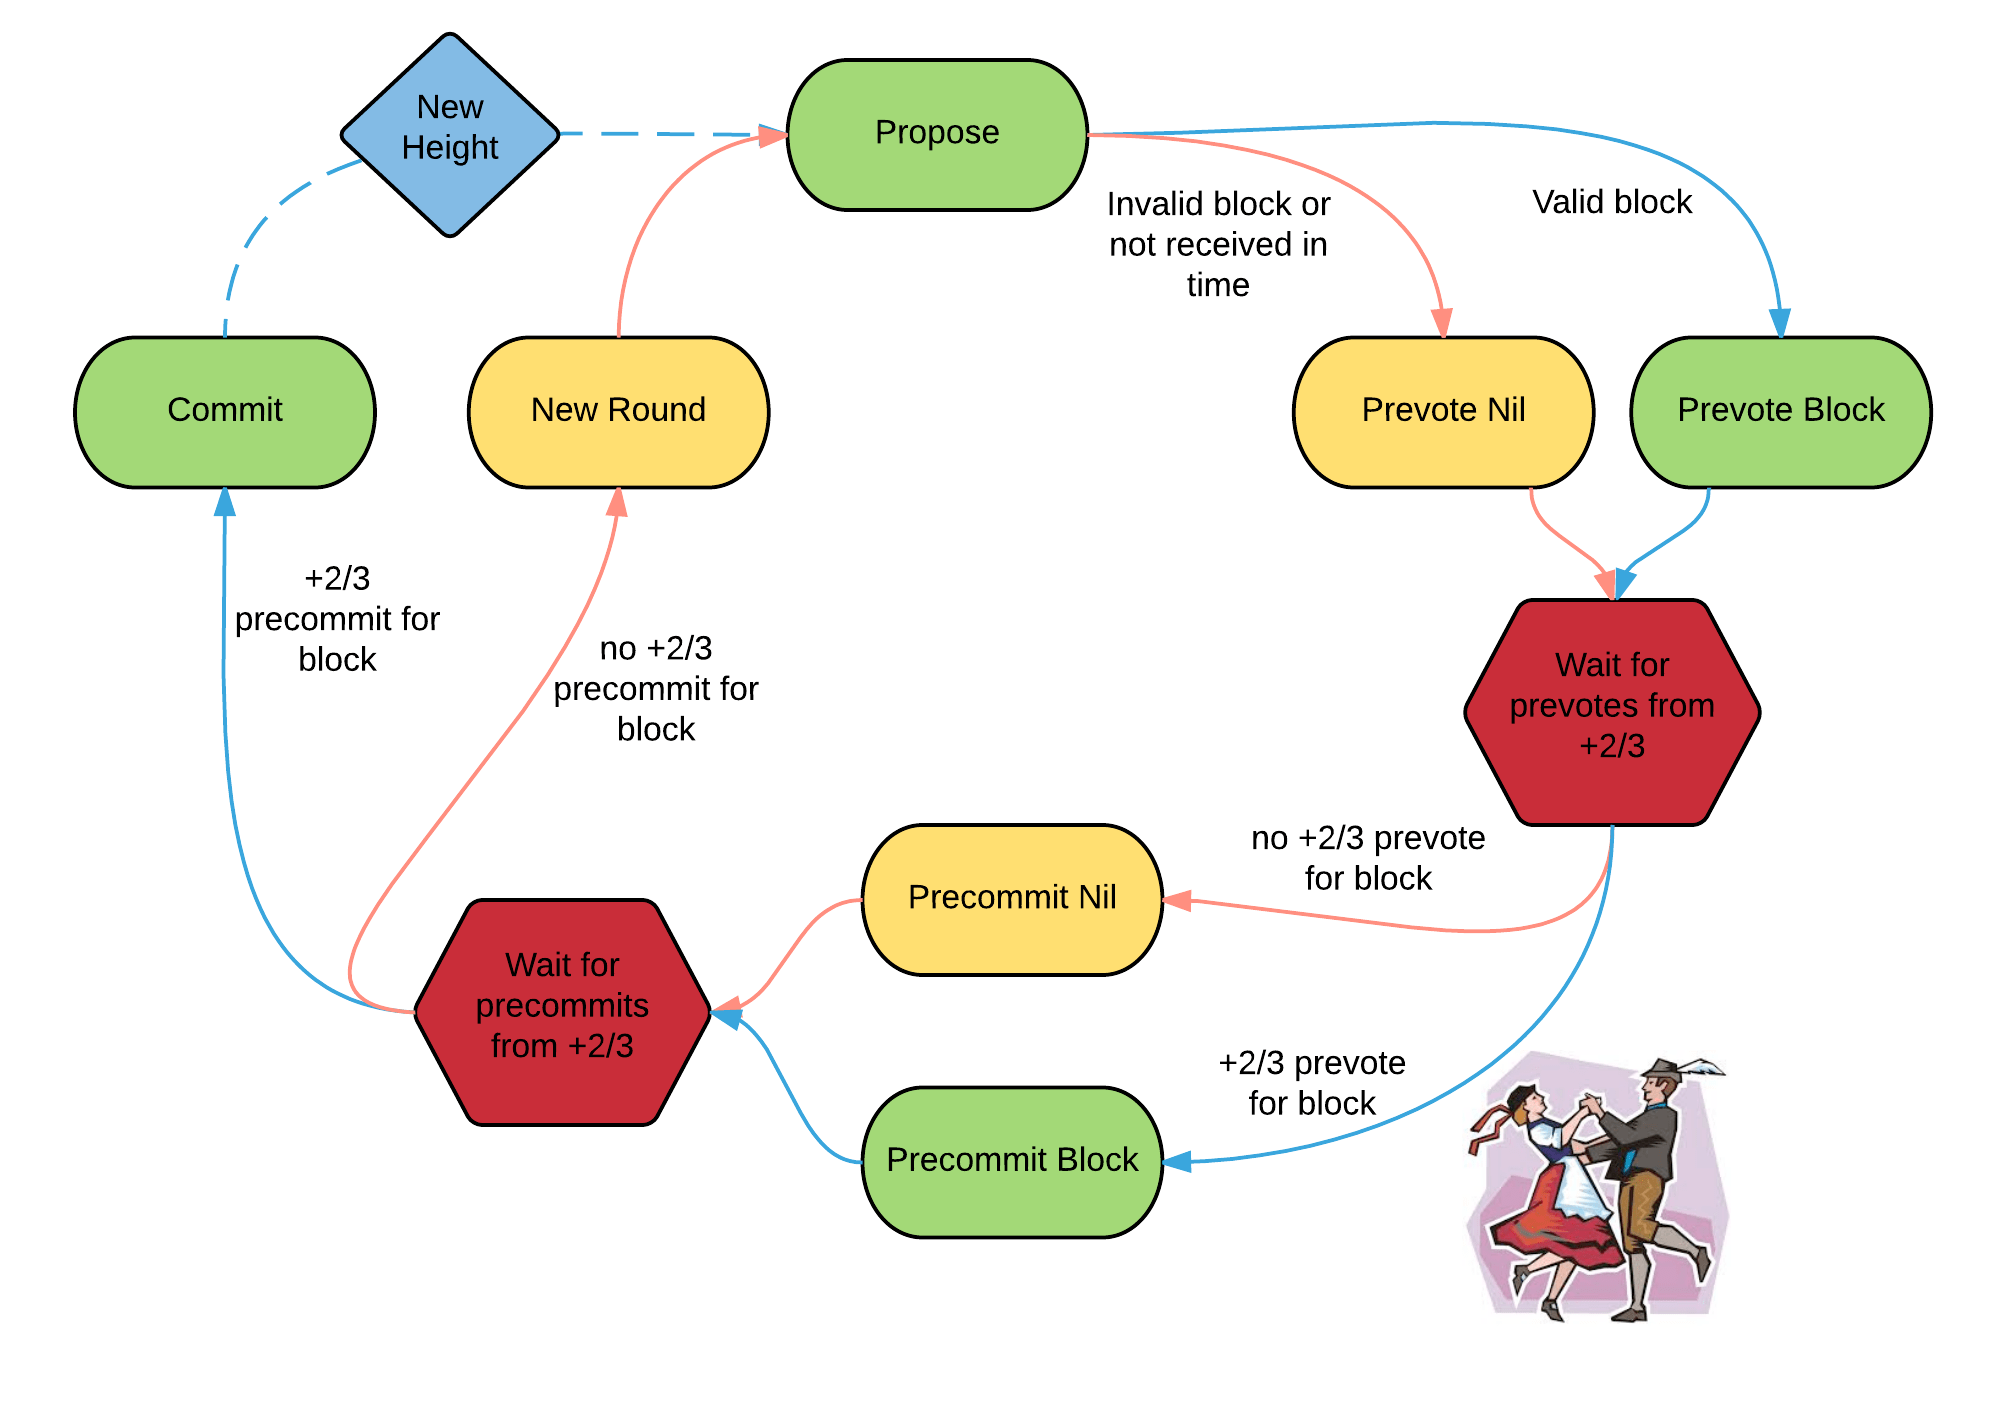
\includegraphics[scale=.15,clip=false]{pictures/polka.png}
  \end{center}

\end{frame}

\begin{frame}\frametitle{Proof of stake: can we trust it?}

  \begin{greenbox}{Yes we can: Ethereum successfully moved from PoW to PoS}
    \begin{itemize}
    \item it's a special case, whose coin ETH is very valuable: validators are a serious form of investment
    \end{itemize}
  \end{greenbox}

  \bigskip
  
  \begin{redbox}{No we can't: all new blockchain projects remain borderline}
    \begin{itemize}
    \item validators initially have no interest in being validators (the coin has no value)
    \item validators are afraid of having a machine always connected and open to the internet
    \item validators find it expensive to maintain and update their machine
    \item validators lose cryptocurrency if a blackout or network failure isolate their machine
    \item please ask this question: ``How many validators your blockchain project has, where are they and who maintains such machines'' (spoiler: very few, in the same room, all maintained by one person)
    \end{itemize}
  \end{redbox}

\end{frame}

\begin{frame}\frametitle{A layered implementation in Golang}

  \begin{center}
    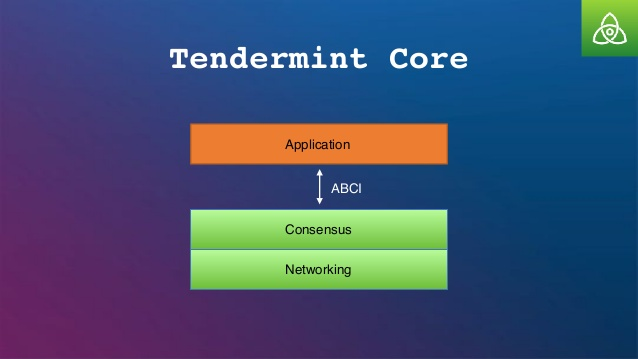
\includegraphics[scale=.38,clip=false]{pictures/tendermint-core.jpg}
  \end{center}

  \smallskip

  ABCI: Application BlockChain Interface

  \smallskip

  This could be done for PoW as well but... nobody did it yet!
  
\end{frame}

\begin{frame}\frametitle{Proof of space}

  \begin{itemize}
  \item proof of work is too expensive and polluting
  \item proof of stake is rather centralized and hard to maintain
  \end{itemize}

  \bigskip

  \begin{greenbox}{Proof of space}
    \begin{itemize}
    \item Ateniese, Bonacina, Faonio, Galesi: \emph{Proofs of Space: When Space Is of the Essence}, 2014 (DAG pebbling)
    \item Dziembowski, Faust, Kolmogorov, Pietrzak: \emph{Proofs of Space}, 2015 (DAG pebbling) $\Rightarrow$
      {\color{red}SpaceMint}: \url{https://github.com/kwonalbert/spacemint}
    \item Abusalah, Alwen, Cohen, Khilko, Pietrzak, Reyzin: \emph{Beyond Hellman's Time-Memory Trade-Offs with Applications to Proofs of Space}, 2017 (proof of sequential work + proof of space) $\Rightarrow$ {\color{red}Chia}: \url{https://www.chia.net/wp-content/uploads/2022/07/ChiaGreenPaper.pdf}
    \item \emph{Signum Community Website and Documentation Project} (plot files) $\Rightarrow$ {\color{red}Signum}: \url{https://wiki.signum.network/signum-plotting-technical-information/index.htm}
    \end{itemize}
  \end{greenbox}
  
\end{frame}

\begin{frame}\frametitle{Proof of space: the general idea}

  \begin{itemize}
  \item each block must report an answer to a \emph{challenge}
  \item the computation of the answer is cheap in time but requires to allocate a large amount of disk space
  \item the quality of the answer determines which block will determine the main chain
  \item the quality of the answer cannot be significantly improved by extra computational work (no time-memory trade-offs)
  \end{itemize}
  
\end{frame}

\begin{frame}\frametitle{Proof of space: Implementations}

  \begin{center}
    {\small\begin{tabular}{c|c|c|c|c|c|c|c}
      name & PoSp? & cons.\ & netw.\ & generic & formalized & since & status \\\hline\hline
      SpaceMint & yes & no & no & no & yes & 2015 & discontinued\\\hline
      Chia & mixed & yes & yes & no & yes & 2017 & active\\\hline
      Signum & yes & yes & yes & no & no & 2014 & active\\\hline
    \end{tabular}}
  \end{center}
  
\end{frame}

\begin{frame}\frametitle{Why Signum?}

  \begin{greenbox}{Pros}
    \begin{itemize}
    \item very simple protocol and algorithm
    \item running since 2014
    \end{itemize}
  \end{greenbox}

  \bigskip

  \begin{greenbox}{Cons}
    \begin{itemize}
    \item in principle, it could be mined by PoW (but never occurred up to now because it would be too expensive
      against its PoSp version: this might change with ASICs)
    \item no formalization, no proofs $\Rightarrow$ suspected attacks (block grinding, time-memory trade-offs)
    \item monolithic, uncommented, chaotic source code
    \end{itemize}
  \end{greenbox}
    
\end{frame}

\begin{frame}\frametitle{A formalization of Signum}

  \begin{greenbox}{}
    Spoto: \emph{A Formalization of Signum's Consensus},
    9th Workshop on Trusted Smart Contracts, 2025, to appear
  \end{greenbox}

  \bigskip

  \begin{itemize}
  \item it clarifies how Signum works
  \item it proves that the suspected block-grinding attack cannot occur
  \item it proves that the suspected time-memory trade-off does not exist (but others might exist! A general proof is still missing)
  \item it proves that Signum does not suffer from challenge-grinding attacks
  \item it introduces a new protection for Signum, against newborn attacks
  \end{itemize}
  
\end{frame}

\begin{frame}{Mokamint}

  Signum is monolithic, uncommented, Java 5, undocumented code

  \bigskip
  \bigskip

  \begin{greenbox}{The idea of Mokamint (Fausto Spoto, March 2023 -- December 2024)}
    \begin{itemize}
    \item Mokamint: a generic blockchain engine based on proof of space
    \item strove for the cleanest architecture
    \item Java 21, modular architecture
    \item open-source, Apache 2.0
    \item integrates with the Takamaka runtime for smart contracts
    \item first network will be published by September 2025
    \item \url{https://github.com/Mokamint-chain/mokamint}
      \begin{center}
        
\includegraphics[scale=0.08,clip=false]{pictures/mokamint_colors.jpg}
      \end{center}
    \end{itemize}
  \end{greenbox}

\end{frame}

\begin{frame}\frametitle{The final picture}

  \begin{center}
    \begin{tabular}{c||c|c}
      PoW & decentralized, energy intensive & direct democracy \\\hline
      PoS & centralized, low energy consumption & (benevolent?) oligarchy \\\hline
      PoSp & decentralized, low energy consumption & direct democracy
    \end{tabular}
  \end{center}
  
\end{frame}

\end{document}
